\documentclass[12pt, french]{article}

\usepackage{fancyhdr, fancybox, lastpage}
\usepackage[most]{tcolorbox}
\usepackage[a4paper, margin={0.3in, .75in}]{geometry}
\usepackage{wrapfig}
\pagestyle{fancy}
\renewcommand\headrulewidth{1pt}
\renewcommand\footrulewidth{1pt}
\fancyhf{}
\rhead{ \em{Zakaria Haouzan}}
\lhead[C]{\em{2ème année baccalauréat Sciences Mathématiques}}
\chead[C]{}
\rfoot[C]{}
\lfoot[R]{}
\cfoot[]{\em{Page \thepage / \pageref{LastPage}}}


\newtcolorbox{Box2}[2][]{
                lower separated=false,
                colback=white,
colframe=white!20!black,fonttitle=\bfseries,
colbacktitle=white!30!gray,
coltitle=black,
enhanced,
attach boxed title to top left={yshift=-0.1in,xshift=0.15in},
title=#2,#1}


\begin{document}
\begin{center}

	\shadowbox { \vspace{-1cm}\bf{Les Ondes mécaniques progressives périodiques}}
\end{center}

\vspace{-0.4cm}
%%_________________________Exercice ! :"_________________________Exercice
   \begin{Box2}{Exercice 1 :  la propagation d’une onde le long d’une corde}
On considère l'aspect d'une corde à l'instant t1 avec une échelle réelle.

  \begin{center}
	  \vspace{-0.2cm}
	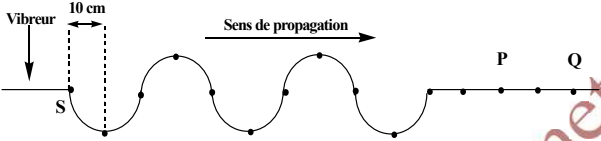
\includegraphics[width=0.48\textwidth]{./img/ex1.png}
  \end{center}

A l'instant t = 0, la source S commence à vibrer avec une fréquence N = 100 Hz. 

1. Calculer la vitesse de l'onde.

2. Trouver la valeur de $t_1$. 

3. Décrire le mouvement de la source S à partir de l'instant t = 0.

4. Trouver toutes les fréquences $N_e$ du stroboscope qui nous permet de visualiser la périodicité spatiale sachant que $N_e > 15 Hz$.

5. Comparer le mouvement des deux points P et Q par rapport à la source S.

6. Représenter, dans le même graphe, les amplitudes des points S et Q.

   \end{Box2}


%%_________________________Exercice !2 :"_________________________Exercice
\begin{Box2}{Exercice 2 :   la propagation d’une onde dans un liquide }
\begin{wrapfigure}{r}{0.26\textwidth}
  \begin{center}
	  \vspace{-1cm}
	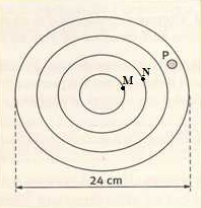
\includegraphics[width=0.24\textwidth]{./img/ex2.png}
  \end{center}
\end{wrapfigure}
Voici l'aspect à l'instant t de la surface d'un liquide où
se propage une onde progressive sinusoïdale. Les cercles
correspondent aux maxima de la perturbation.
Au point P se trouve un petit flotteur qui est animé
d'un mouvement de fréquence 7,5 Hz.

1. Calculer la célérité des ondes.

2. Comparer le mouvement entre les points M et N puis entre les points N et P en déduire.

\end{Box2}

%%_________________________Exercice ! 3:"_________________________Exercice
\begin{Box2}{Exercice 3 :la célérité du son. }
\begin{wrapfigure}{r}{0.28\textwidth}
  \begin{center}
	  \vspace{-0.8cm}
	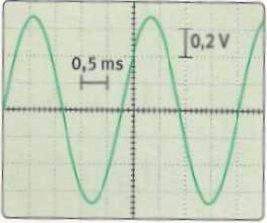
\includegraphics[width=0.28\textwidth]{./img/ex3.png}
  \end{center}
\end{wrapfigure}
On enregistre à l'aide d'un microphone relié à un oscilloscope le son émis par un
diapason.

1. Caractériser l'onde émise par la diapason.

2. Déduire de la courbe obtenue la fréquence de
son émis.

3. Décrire un mode opératoire permettant à
l'aide d'un second microphone, relié à l'autre
voie de l'oscilloscope, de mesurer la longueur
d'onde du signal sonore émis par le diapason.

4. On obtient $\lambda = 77 cm$. En déduire la
célérité du son.

5. En répétant l'expérience avec un autre
diapason qui produit un son de fréquence
$f = 330 Hz$, on mesure une longueur d'onde
$\lambda= 1m$. Commenter.

\end{Box2}

%%_________________________Exercice 4 : _________________________Exercice
\begin{Box2}{Exercice 4 :corde élastique }
	Un vibreur provoque des ondes sinusoïdales de fréquence $f=50Hz$ à l'extrémité d'une corde. 

	Un point M situé à la distance $d=18cm$ de l'extrémité commence à vibrer à l'instant $t=0,060s$ après la mise en fonction du vibreur.

1. Déterminer la célérité des ondes le long de cette corde.
2. Représenter sur deux graphes différents l'évolution de la position du point M et celle de la source S pour t
variant de 0 à 0,080s.

3. Comparer l'état vibratoire du point M et du point S. Que peut-on dire de la distance les séparant.

4. Quelle est la plus petite distance séparant deux points vibrant en phase?

5. Pour quelle fréquence la distance précédente vaut- elle 5cm?
\end{Box2}


\begin{Box2}{Exercice 5 :Périodicité temporelle }
%\begin{wrapfigure}{r}{0.4\textwidth}
  %\begin{center}
	  %\vspace{-0.6cm}
	%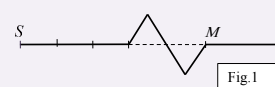
\includegraphics[width=0.4\textwidth]{./img/Ex4}
  %\end{center}
%\end{wrapfigure}

Deux haut-parleurs identiques $H_1$ et $H_2$ sont alimentés par un même GBF. 
Le haut-parleurs $H_1$, adapté à cet usage, est immergé dans l'eau, tandis que $H_2$ est à l'air libre. 

On place un microphone $M_1$ face au haut-parleurs $H_1$, à une distance $d_1$, et un microphone $M_2$ face au haut-parleurs $H_2$, à une distance $d_2$. 

Les microphones $M_1$ et $M_2$ sont reliés en voies 1 et 2 d'un oscilloscope.

La vitesse du son est de $340 m/s$ dans l'air, et de $1500 m/s$ dans l'eau dans les conditions de l'expérience.

La fréquence du signal sinusoïdale délivré par le GBF est f = 1 kHz.

\textbf{1. }Quelle est la plus petite valeur $d_{1min}$ non nulle de $d_1$ pour que $M_1$ et $H_1$ soient en phase.

\textbf{2. }On déplace le microphone $M_2$ jusqu'à ce que $d_1=d_{1min}$. 

Calculer le retard $\tau$ avec lequel le son arrive $M_2$. Représenter les courbes obtenus pour le l'oscilloscope pour une vitesse de balayage de 1 ms/div.

\textbf{3. }Quelle distance minimale doit séparer $M_2$ et $H_2$ pour que es deux courbes soient en phrase?

\end{Box2}
%\vspace{2cm}
\begin{center}
   \Large{ \em{Exercices Supplémentaires}}
\end{center}


%\vspace{-0.7cm}
%%_________________________Exercice 5 : _________________________Exercice
\begin{Box2}{Exercice 6 :Propagation d’une onde mécanique à la surface de l’eau  }
On crée, à l’instant $t_0$, en un point S de la surface de l’eau, une onde mécanique progressive sinusoïdale
de fréquence N = 50 Hz

La figure ci-dessous représente une coupe verticale de la surface de l’eau à un instant t. La règle
graduée sur le schéma indique l’échelle utilisée.

\begin{center}
	  %\vspace{-0.6cm}
	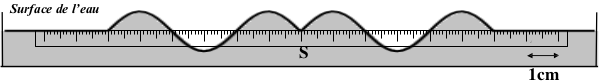
\includegraphics[width=1\textwidth]{./img/ex6.png}
  \end{center}

Déterminer :
\begin{enumerate}
	\item  Longueur d’onde

	\item  La vitesse de propagation de l’onde à la surface de l’eau,

	\item  L’instant t, où la coupe de la surface de l’eau est représentée,

	\item  On considère un point M de la surface de l’eau, éloigné de la source S d’une distance $SM = 6cm$. Le point M reprend le même mouvement que celui de S avec un retard temporel $\tau$ . écrire
la relation entre l’élongation du point M et celle de la source S ?
\end{enumerate}
\end{Box2}
%%_________________________Exercice 6 : _________________________Exercice
%\begin{Box2}{Exercice 6 : échographie}
%%\begin{wrapfigure}{r}{0.2\textwidth}
  %%\begin{center}
	  %%\vspace{-0.6cm}
	%%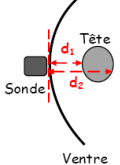
\includegraphics[width=0.2\textwidth]{./img/Exercice6.png}
  %%\end{center}
%%\end{wrapfigure}
%6
%\end{Box2}

\end{document}
